%!TEX root = ../thesis_a4.tex

\chapter{Background}
\label{chap:background}

\section{Introduction}

In this chapter we provide the relevant music and scientific background for the work presented in this dissertation. We start with a brief discussion on the terminology used in this thesis (\secref{sec:background_terminology}). Subsequently, we provide an overview of the selected music concepts relevant to better understand our work (\secref{sec:music_background}). We then present a review of the literature related with the topics addressed in this thesis. We first present relevant work done in computational analysis of \gls{iam} (SEction XX), which includes approaches for tonic identification, automatic \gls{raga} recognition and melodic pattern processing. Then, we present work done for other music traditions within \gls{mir} on topics covering melodic pattern processing and key recognition (\secref{sec:background_relevant_work_other_music}). Finally, we provide an overview of the select scientific concepts in information retrieval, time-series analysis, complex networks and statistics (\secref{sec:background_scientific_background}). We conclude this chapter by providing a summary of the literature review, wherein we highlight the shortcomings of the existing approaches, and identify some possible venues for scientific contribution (\secref{sec:background_summary}). 

\section{Terminology}
\label{sec:background_terminology}

In this section we provide working definition of the selected terms we have used throughout the thesis. Since the thesis focuses on the melodic description of \gls{iam}, it is important to clearly understand the meaning of melody in the context of this thesis. Our aim here is not to formally define melody in an universal sense, which as we see from the literature has been a challenge in itself, with almost every definition falling short of considering some aspect or the other XXXX. It would not be an overstatement to say that there is no agreed definition of melody that suits every context. For a review of interesting definitions of melody we refer to XXXX. Before we present the definition of melody that we consider in this work, it is important to understand the performance or concert setup in \gls{iam}. Since this music tradition is performance-based, even the studio recordings follow the same setup. Performances in \gls{iam} have a clearly defined concept of a lead artist, who plays the central role (also literally positioned in the center of the stage) and all other instruments are considered the accompaniments. In this context, mergin relevant parts of the definitions given by~\cite{paiva2006melody,kim2000analysis,levitin2002memory} covers to a large extent the scope of melody in \gls{iam}. Their definitions in the respective order are: \textquote{``\textit{the dominant individual pitched line in a musical ensemble}''} and \textquote{``\textit{an auditory object that emerges from a series of transformations along the six dimensions: pitch, tempo, timbre, loudness, spatial location, and reverberant environment}''}.  The first definition falls short of considering several other dimensions of sound such as timbre and loudness that are important in perception and production of melody, which are taken into account in the second definition. The concept of audio as a mixture of sounds from multiple instruments (`\textit{ensemble}') is missing in the second definition, which the first definition takes into account. The idea of continuity and smoothness of melody is expressed by `\textit{line}' in the former and by `\textit{series of transformations}' in the latter. If we combine these two definitions we can rewrite our working definition as \textquote{``\textit{an auditory object that emerges from a continuous series of transformations along the six dimensions: pitch, tempo, timbre, loudness, spatial location, and reverberant environment, by the dominant individual sound source in a music ensemble}''}. Although, we only consider the pitch dimension of melody in this thesis. Thus, loosely speaking, for all practical purposes within the scope of this thesis, we represent melody by a continuous pitch time-series corresponding to the lead artist in an audio recording, also referred to as predominant pitch in the subsequent chapters. This definition does not explicitly take into account the rare case of two lead artists. Since in a majority of such cases the two lead sound sources are active sequentially in time, our definition encompasses this scenario by considering the active sound source as dominant. \TODO{please make this shit better, these thigns are so confusing and broad}

Now that we have a working definition of melody, we proceed to define the scope of the terms such as melodic patterns, phrases and motifs in this thesis, and disambiguate them with other seemingly synonymous terms such as melodic fragment and segment. Melodic fragment or melodic segment in this thesis refers to a continuous subsequence of the pitch sequence. It does not entail any musical relevance in terms of the boundaries or the length of the subsequence. By a melodic pattern we refer to a repeating melodic fragment, where the scope and the meaning of repetition is based on the perceived melodic similarity. Across repetitions, a melodic fragment can undergo a series of time and pitch transformations allowed within the periphery of melodic framework (\gls{raga} in our case) without altering the identity of the melodic unit. Also, the melodic similarity here refers to the perceived similarity between melodic fragments when heard in isolation, as the local melodic context can influence the perception of similarity. Melodic patterns in this thesis do not entail any particular musical significance in terms them being characteristic of a melodic concept in \gls{iam}. The terms melodic pattens, fragments and segments are more from the perspective of signal or the time-series. Melodic phrases on the other hand are used in the context of music, as being a unit of melody which encapsulate an idea or a musical thought by an artist. Melodic motif is further high-level concept and we use it to refer to a particular type of characteristic patterns, in out thesis of \glspl{raga}, \gls{raga} motifs. 


The word polyphonic in the context of audio recordings signifies that the recordings consists of a mixtue of multiple instruments playing simultaneously.


\section{Music Background}
\label{sec:music_background}

\subsection{Indian Art Music}

\subsection{Melodies in Indian Art Music}

\subsubsection{Tonic in Indian art music}
\label{sec:background_tonic_in_iam}

\subsubsection{Svaras}

\subsubsection{Aroh-Avroh}

\subsubsection{Gamakas and Ornaments}

\subsubsection{Raga in Indian Art Music}

\paragraph{Phase-based and Scale-based ragas}
\paragraph{Allied ragas}

\subsubsection{Characteristic Melodic Phrases}

\subsubsection{Chalan}

\subsubsection{Nyas}
\label{sec:backgroung_nyas_description}

Dey presents various interpretations and perspectives on the concept of ny\={a}s in Hindustani music according to ancient, medieval and modern authors~\cite{Dey2008}. In the context of its current form, the author describes ny\={a}s as that process in a performance of a r\={a}g where an artist pauses on a particular svar\footnote{The seven solf\`{e}ge symbols used in Indian art music are termed as svars. It is analogous to note in western music but conceptually different.}, in order to build and subsequently sustain the format of a r\={a}g, the melodic framework in Indian art music~\cite[p. 70]{Dey2008}\cite{KKG_SS13}. Dey elaborates the concept of ny\={a}s in terms of action, subject, medium, purpose and effect associated with it. Typically, occurrence of a ny\={a}s delimits melodic phrases (motifs), which constitute one of the most important characteristic of a r\={a}g. Analysis of ny\={a}s is thus a crucial step towards melodic analysis of Hindustani music. In particular, automatically detecting occurrences of ny\={a}s (from now on referred as ny\={a}s segments) will aid in computational analyses such as melody segmentation, motif discovery, r\={a}g recognition and music transcription~\cite{GopalJNMR2012, Rao2014}. However, detection of ny\={a}s segments is a challenging computational task, as the prescriptive definition of ny\={a}s is very broad, and there are no fixed set of explicit rules to quantify this concept~\cite[p. 73]{Dey2008}. It is through rigorous practice that a seasoned artist acquires perfection in the usage of ny\={a}s, complying to the r\={a}g grammar and exploring creativity through improvisation at the same time. 

\subsubsection{Recurring Melodic Patterns in IAM}


\section{Relevant Work in Indian Art Music}
\label{sec:background_relevant_work_iam}


\subsection{Tonic Identification}
\label{sec:background_relevant_work_tonic_identification}

Identification of tonic pitch of the lead artist in an audio recording is a crucial first step in tonal analysis of \gls{iam} (\secref{sec:background_tonic_in_iam}). Knowing the tonic pitch used in an audio recording enables a meaningful comparison of melodies across different artists and their recordings. In this section we review existing approaches for automatic tonic identification in audio collections of \gls{iam}. 

As mentioned, there have been various efforts to automatically identify the tonic pitch of the lead artist in a performance of Indian art music~\citep{salamon2012multipitch,gulati2012two,bellur2012knowledge,ranjani2011carnatic,Sengupta2005b}. These approaches mainly differ in terms of the musical cues that they utilize to identify the tonic, the amount of input audio data used to perform this task and the type of music material they are devised for (Hindustani or Carnatic, vocal or
instrumental, etc.). Despite the differences, all these approaches can be divided into three main processing blocks, as shown in~\figref{fig:tonic_identification_general_block_diagram}. The only exception to this schema is the approach proposed by~\cite{Sengupta2005b}.

\begin{figure}
	\begin{center}
		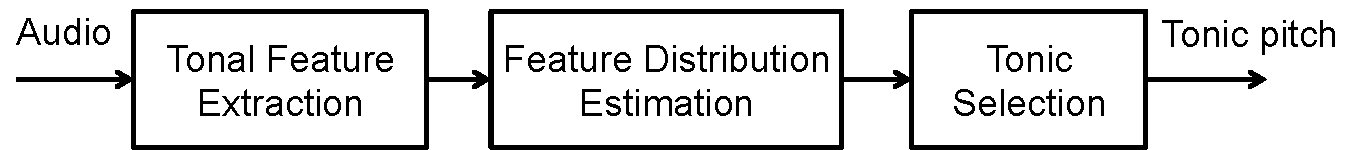
\includegraphics[width=\figSizeNinety]{ch05_preprocessing/figures/tonic_identification_block_diagram.pdf}
	\end{center}
	\caption[General block diagram of the processing steps used by tonic identification
	approaches.]{General block diagram of the processing steps used by tonic identification
		approaches.}
	\label{fig:tonic_identification_general_block_diagram}
\end{figure}


In all the aforementioned approaches, the three main processing blocks are the following: feature extraction, feature distribution estimation and tonic selection. Since the task of tonic identification involves an analysis of the tonal content of the audio signal, the features extracted in the first block are always pitch related. In the second block, an estimate of the distribution of these features is obtained using either Parzen window based density estimation or by constructing a histogram. The feature distribution is then used in the third block to identify the tonic. The peaks of the distribution correspond to the most salient pitch values used in the performance (usually the \glspl{svara} of the \gls{raga}), one of which corresponds to the tonic pitch. As the most salient peak in the distribution is not guaranteed to be the tonic, various techniques are applied to select the peak that corresponds to the tonic.

{\renewcommand{\arraystretch}{1.5}
	\begin{sidewaystable} 
		\begin{centering}
			\begin{tabular}{ c c c c }
				\tabletop			
				Method 	&	Features	&	Feature Distribution	&	Tonic Selection \\
				\tablemid			
				\acrshort{tonicid_sengupta} \citep{Sengupta2005b}	&	Pitch \citep{AKDatta_1996} & N/A & Error minimization\\
				
				\acrshort{tonicid_ranjani_1}/\acrshort{tonicid_ranjani_2} \citep{ranjani2011carnatic}	&	Pitch \citep{BoersmaPaul2001} & Parzen-window-based \acrshort{pde}  & GMM fitting\\
				
				\acrshort{tonicid_justin} \citep{salamon2012multipitch} & Multi-pitch salience \citep{Salamon2011} & Multi-pitch histogram & Decision tree\\
				
				\acrshort{tonicid_sankalp} \citep{gulati2012two}	& Multi-pitch salience  \citep{Salamon2011} & Multi-pitch histogram & Decision tree\\
				
				&	Predominant melody \citep{Salamon2012} & Pitch histogram & Decision tree\\
				
				\acrshort{tonicid_ashwin_1} \citep{bellur2012knowledge}	&	Pitch \citep{DeCheveigne2002}	&  \acrshort{gd} histogram & Highest peak\\
				
				\acrshort{tonicid_ashwin_2} \citep{bellur2012knowledge}	&	Pitch \citep{DeCheveigne2002}	& 	GD histogram	&
				Template matching\\
				
				\acrshort{tonicid_ashwin_2} \citep{bellur2012knowledge}	&	Pitch \citep{DeCheveigne2002}	& 	GD histogram
				& Highest peak\\
				
				\acrshort{tonicid_chordia}	& 	& 	& \\			
				
				\tablebot			
			\end{tabular}
			
			\caption[Summary of existing tonic identification approaches.]{Summary of existing tonic identification approaches.}
			\label{tab:pre_processing_tonic_identification_summary_methods}
			\par \end{centering}	
	\end{sidewaystable}
	
	
In \tabref{tab:pre_processing_tonic_identification_summary_methods} we provide a summary of the existing methods for tonic identification. The common processing blocks and the main differences between them become evident from this table. A detailed review of these methods in terms of the three processing stages as shown in \figref{fig:tonic_identification_general_block_diagram} is done in~\cite{Gulati2014Tonic}. For a more detailed description of these methods we refer to their respective publications listed in Table \tabref{tab:pre_processing_tonic_identification_summary_methods}. 




\subsection{R\={a}ga Recognition}

\subsection{Melodic Pattern Processing}



\section{Relevant Work (in MIR??) or (Other Music Tradition?)}
\label{sec:background_relevant_work_other_music}

\subsection{Key and Mode Recognition}

\subsection{Pattern Processing in Music}

% Patterns at different time scales: 1) Sections, 2) Motifs, 3) Stanzas 4) Chord sequences? 

% Focus on Motifs/Riffs 

% Subparts: Melody representation, Melody segmentation, Melodic similarity, Discovery methodology, Redundancy reduction etc

\subsection{Corpus level melodic analysis}

%SOME MATERIAL FOR THIS CHAPTER (IN NO ORDER)

%In computational analysis of \gls{iam}, \gls{nyas} segment detection has not received much attention in the past. To the best of our knowledge, only one study with the final goal of spotting melodic motifs has indirectly dealt with this task~\citep{Ross2012}. In it, the authors considered performances of a single r\={a}g and focused on a very specific \gls{nyas} \gls{svara}, corresponding to a single scale degree: the fifth with respect to the tonic, the `Pa' \gls{svara}. This \gls{svara} is considered as one of the most stable \glspl{svara}, and has minimal pitch deviations. Thus, focusing on it oversimplified the methodology developed in~\cite{Ross2012} for \gls{nyas} segment detection. \TODO{Should we move this to state of the art? + svara notation should be replaced by a glossary item?} 
%
%A related topic is the detection of specific \glspl{alankar} and characteristic phrases (also referred as {\it Pakads}) in melodies in Indian art music~\cite{Datta2007, Pratyush2010, Ross2012b, Ishwar2013}. These approaches typically exploit pattern recognition techniques and a set of pre-defined melodic templates. A nearest neighbors classifier with a similarity measure based on dynamic time warping (DTW) is a common method to detect patterns in melodic sequences~\cite{Pratyush2010, Ross2012b}. In addition, it is also the most accurate~\cite{Xi06ICML} and extensively used approach for time series classification in general (cf.~\cite{Wang12DMKD}). Notice that the concept of landmark has been used elsewhere, with related but different notions and purposes. That is the case with time series similarity~\cite{Perng00ICDE}, speech recognition~\cite{Jansen08JASA,Chen12ICASSP}, or audio identification~\cite{Duong13ICASSP}.


%
%\section{Motif discovery in time-series}
%\subsection{Lower-bounding techniques for DTW}
\section{Scientific Background}
\label{sec:background_scientific_background}

\subsection{Distance Measures}
\subsubsection{Euclidean Distance}
\subsubsection{Dynamic Time Warping}
\subsubsection{KL Divergence}
\subsubsection{Bhattacharya}

\subsection{Indexing of Time-series}
\subsubsection{Lower Bounds for DTW distance}

\subsection{Evaluation Measures for Information Retrieval}
\subsubsection{Precision and Recall}
\subsubsection{Mean Average Precision}
\subsubsection{Expert Evaluation?}

\subsection{Machine Learning Concepts}
\subsubsection{Classification Methods}
\subsubsection{Evaluation Strategies}

\subsection{Complex Networks}


\subsection{Statistical Testing}
\subsubsection{Mann-Whitney U Test}
\subsubsection{Wilcoxin Test}
\subsubsection{Signed Rank Test}
\subsubsection{McNemar's Test}
\subsubsection{Holm-Bonferroni Method}


\section{Summary}
\label{sec:background_summary}
